\documentclass[9pt,pdf,utf8,hyperref={unicode},aspectratio=169]{beamer}

%Привычный шрифт для математических формул
\usefonttheme[onlymath]{serif}
\mode<presentation>
{
    \usetheme{boxes}
    \beamertemplatenavigationsymbolsempty

    \setbeamercovered{transparent}
    \setbeamertemplate{navigation symbols}{}
    
    \setbeamertemplate{footline}[frame number]
    \setbeamertemplate{caption}[numbered]
    % \setbeamersize{text margin left=0.5em, text margin right=0.5em}
}

% Дополнительные библиотеки
\usepackage[T2A]{fontenc}
\usepackage[english, russian]{babel}
\usepackage[utf8]{inputenc}
\usepackage{amsmath,amssymb}
\usepackage{indentfirst}
\usepackage{changepage}
\usepackage{enumerate}
\usepackage{mathtools}
\usepackage{multicol}
\usepackage{multirow}
\usepackage{ragged2e}
\usepackage{multicol}
\usepackage{diagbox}
\usepackage{wrapfig}
\usepackage{comment}
\usepackage{subfig}
\usepackage{array}
\usepackage{color}
\usepackage{tikz}
\usepackage{url}
\usepackage{bm}

\usetikzlibrary{trees}

% Определение дополнительных функций
\DeclareMathOperator*{\plim}{\mathop{plim}}
\DeclareMathOperator{\prob}{\mathbf{P}\!}

\DeclareMathOperator{\arctanh}{arctanh}
\DeclareMathOperator{\mmode}{mode}
\DeclareMathOperator{\rank}{rank}
\DeclareMathOperator{\diag}{diag}
\DeclareMathOperator{\sign}{sign}
\DeclareMathOperator{\cov}{cov}
\DeclareMathOperator{\pow}{pow}
\DeclareMathOperator{\med}{med}

\def\argmin#1{ \mathop{\text{argmin}}\limits_{#1} }
\def\argmax#1{ \mathop{\text{argmax}}\limits_{#1} }

\newcommand{\tsum}{\mathop{\textstyle\sum}\limits}
\newcommand{\condprob}[2] {\mathbf{P}\!\left(#1\left|#2\right.\right)}

\renewcommand{\leq}{\leqslant}
\renewcommand{\geq}{\geqslant}

\DeclareMathOperator{\FWER}{FWER}
\DeclareMathOperator{\FDR}{FDR}
\newtheorem{Th}{Теорема}
\newtheorem{Def}{Определение}

% Основная часть

\title[Причинность]{Прикладной статистический анализ данных\\Последовательный анализ}
\author{Андрей Грабовой}
\date{}

\begin{document}
\tikzstyle{every node}=[draw=black,thick,anchor=west]
\tikzstyle{selected}=[draw=red,fill=red!30]
\tikzstyle{optional}=[dashed,fill=gray!50]

\begin{frame}
    \titlepage
\end{frame}

\begin{frame}{История задачи}
\begin{block}{Задача}
ВМФ США хочет проверить эффективность двух типов снарядов. Производится $N$ ($N \approx 1000$) раундов обстрелов целей двумя типами снарядов, после чего производится статистический тест.
\end{block}

\begin{block}{Проблема}
Статистический тест может быть слишком расточительным. Часто знающий офицер может ``на глаз'' понять, какой снаряд лучше после нескольких сотен раундов.
\end{block}

\end{frame}

\section{Распределение Бернулли}
\subsection{Одна выборка}
\begin{frame}{Z-критерий меток для доли}
     \only<1>{
     	\textbf{Задача:} рекламная кампания планировалась так, чтобы обеспечить узнаваемость продукта среди целевой аудитории более~30\%. После окончания кампании проводится опрос с целью оценки узнаваемости.
     	
     	\bigskip
     	
     	$H_0\colon$ узнаваемость продукта не превышает 30\%.
     	
     	$H_1\colon$ узнаваемость продукта превышает 30\%.
     }	
	
    \only<2>{
    \begin{center}
        \begin{tabular}{rl}
            выборка:                        & $X^{n}=\left(X_{1},\ldots,X_{n}\right), X \sim Ber\left(p\right)$ \\
            нулевая гипотеза:               & $H_0\colon p=p_0$ \\
            альтернатива:                   & $H_1\colon p>p_0$ \\
            статистика:                     & $Z\left(X^{n}\right) = \frac{\hat{p}-p_0}{\sqrt{\frac{p_0\left(1-p_0\right)}{n}}}, \;\; \hat{p} = \frac1{n}\sum\limits_{i=1}^n X_i$ \\
            нулевое распределение:          & $N(0,1)$\\
        \end{tabular}
        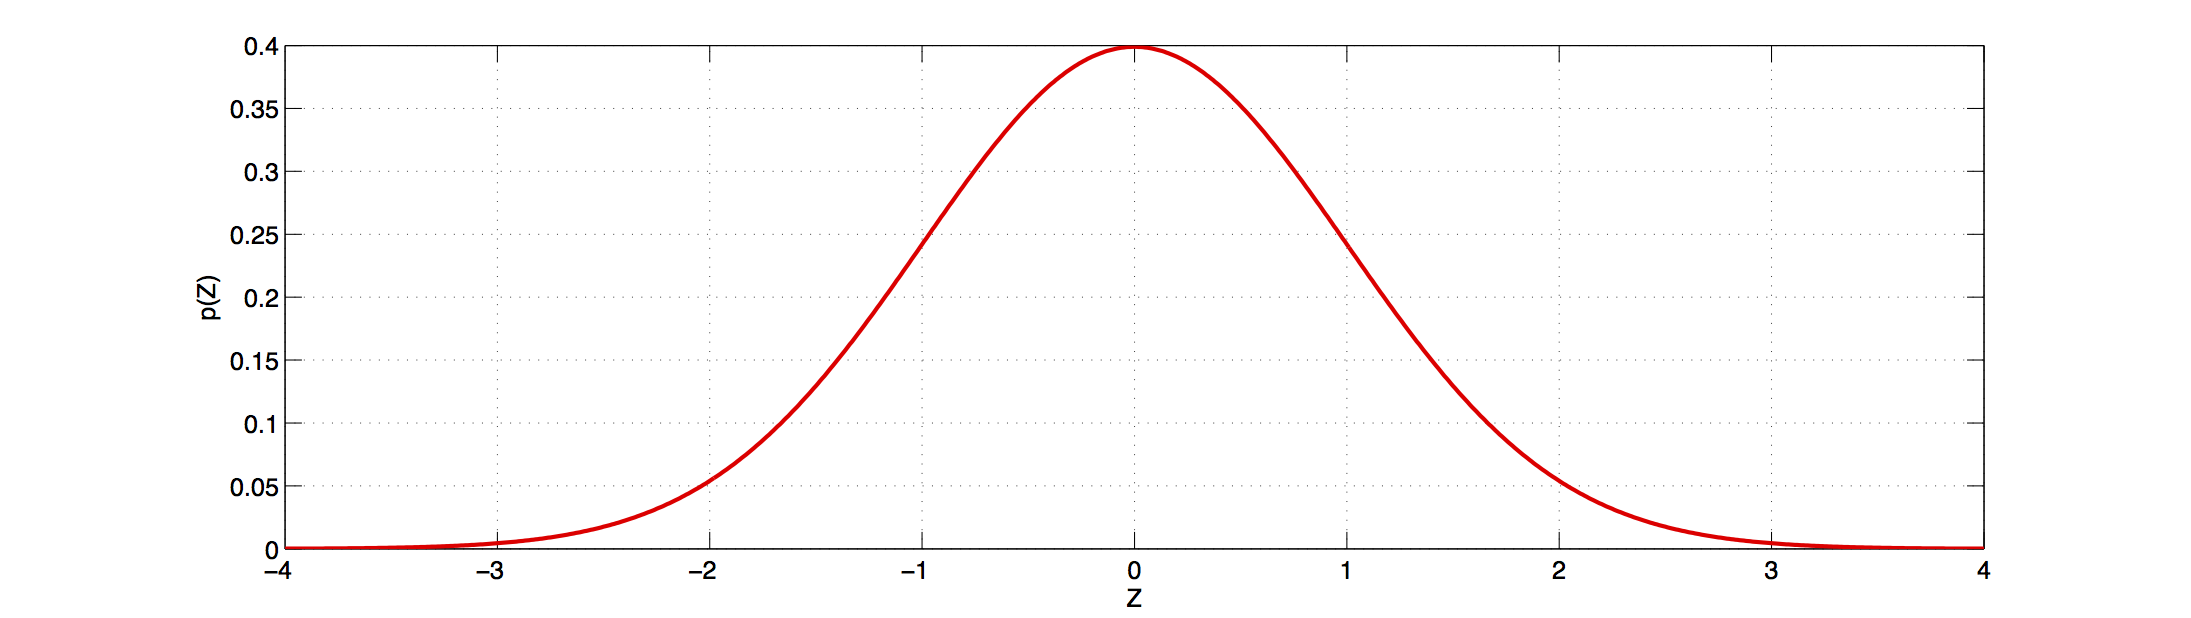
\includegraphics[width=0.85\textwidth]{norm.png}
    \end{center}
     }

    \only<3>{
    \begin{center}
        \begin{tabular}{rl}
            выборка:                        & $X^{n}=\left(X_{1},\ldots,X_{n}\right), X \sim Ber\left(p\right)$ \\
            нулевая гипотеза:               & $H_0\colon p\leq p_0$ \\
            альтернатива:                   & $H_1\colon p>p_0$ \\
            статистика:                     & $Z\left(X^{n}\right) = \frac{\hat{p}-p_0}{\sqrt{\frac{p_0\left(1-p_0\right)}{n}}}, \;\; \hat{p} = \frac1{n}\sum\limits_{i=1}^n X_i $ \\
            нулевое распределение:          & $N(0,1)$ при $p=p_0$ 
        \end{tabular}
        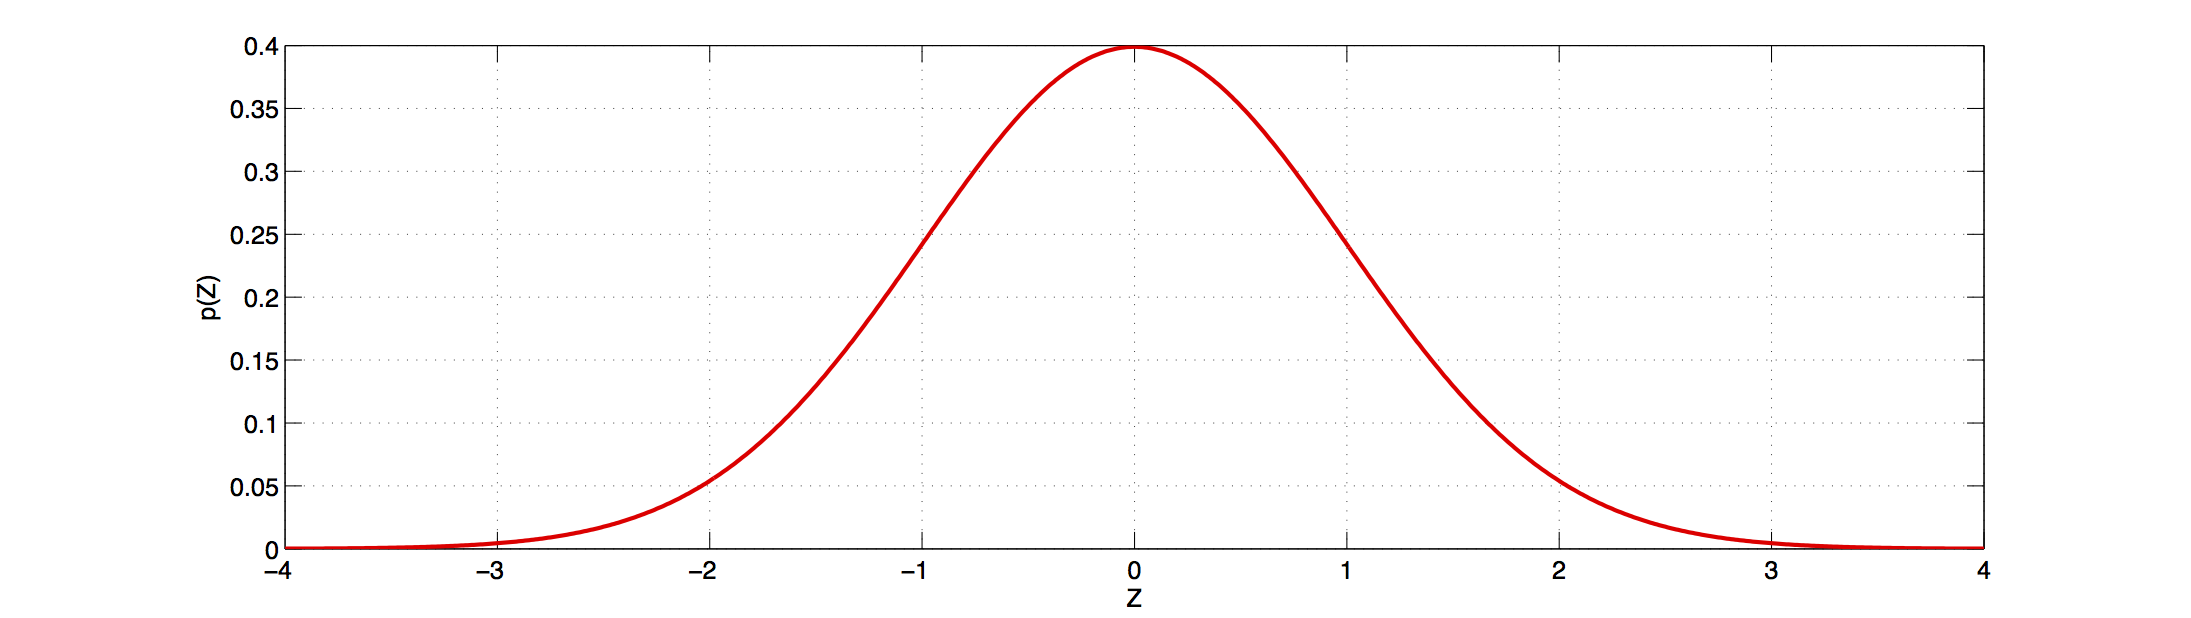
\includegraphics[width=0.85\textwidth]{norm.png}
    \end{center}
     }

     \only<4>{
    Как выбрать наименьший достаточный объём выборки?
     	
     	\bigskip
     	
     }
\end{frame}

\begin{frame}{Последовательный анализ Вальда: ключевая идея}
 \only<1>{
        Вместо порога $p_0$ введем два порога: $p_L, p_U$. Будем полагать, что отклонение значения параметра $p$ от $p_0$ несущественно, если:
           $$p_L\leq p_0\leq p_U.$$

        Алгоритм
        \begin{enumerate}
        \item Если $\frac{p} \geq r_m$ для очередной выборки $x_1,\dots,x_m$: отклонить гипотезу $H_0$.
        \item Если $\frac{p} \leq a_m$ для очередной выборки $x_1,\dots,x_m$: принять гипотезу $H_0$.
        \item Если $a_m<\frac{p} <r_m$, пополнить выборку: $m := m+1$.
        \end{enumerate}
        \begin{center}
        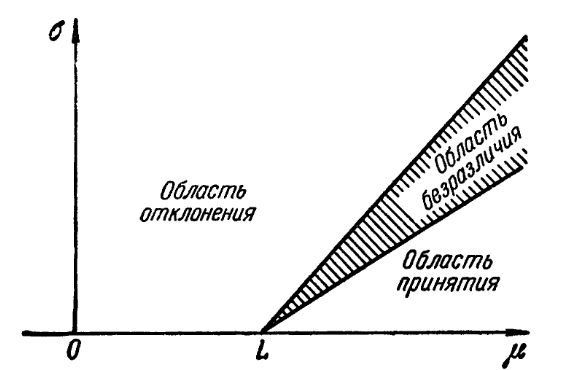
\includegraphics[width=0.35\textwidth]{wald_ru.png}
        \end{center}
        }



 \only<2>{
        Пусть: 

        $\alpha$~--- уровень значимости --- допускаемая вероятность ошибки первого рода,

        $\beta$~--- допускаемая вероятность ошибки второго рода.

        Вероятность получения такой выборки $x_1,\dots,x_n$, что 

        \[
        B<\frac{p_U}{p_L} <A (\text{для меньших подвыборок}), \quad {\frac{p_U}{p_L} \geq A}
        \]
        при выполнении гипотезы $H_1 (p = p_U)$ больше в $A$ раз, чем при выполнении альтернативы $H_0 (p = p_L)$.

        Но эта вероятность равна $\alpha$ при верности $H_0$ и $1 - \beta$ при верности $H_1$:
        \[
        1 - \beta \geq \alpha A.
        \]
        }


\end{frame}



\begin{frame}{Постановка задачи последовательного анализа}
   \begin{center}
        \begin{tabular}{rl}
            выборка:                        & $X^{m}=\left(X_{1},\ldots,X_{m}\right), X \sim Ber\left(p\right).$ \\
        \end{tabular}
   \end{center}

   \bigskip

   Фиксируем <<коридор>> отклонений значения параметра $p$ от $p_0$, которые можно считать несущественными:
   $$p_L\leq p_0\leq p_U$$
   (хотя бы одно из неравенств~--- строгое).

   \bigskip

   \begin{center}
        \begin{tabular}{rl}
            нулевая гипотеза:               & $H_0\colon p\leq p_L;$ \\
            альтернатива:                   & $H_1\colon p\geq p_U.$ \\
        \end{tabular}
   \end{center}

   \bigskip

   Пусть данные поступают постепенно.

   Задача: построить проверку гипотез так, чтобы обойтись как можно меньшим объёмом выборки.
   
   \bigskip
   
   Анонс: процедура последовательного анализа при тех же значениях мощности и уровня значимости позволяет обойтись меньшим (иногда вдвое) объёмом выборки.
\end{frame}

\begin{frame}{Процедура последовательного анализа}
    \only<1>{
    Поскольку размер выборки не фиксирован, мы можем фиксировать вероятности ошибок обоих родов:

    $\alpha$~--- уровень значимости --- допускаемая вероятность ошибки первого рода,

    $\beta$~--- допускаемая вероятность ошибки второго рода.

   \begin{center}
        \begin{tabular}{rl}
            статистика:                        & $d_m\left(X^{m}\right) = \sum\limits_{i=1}^m X_i.$ \\
        \end{tabular}
   \end{center}

    Введём следующие обозначения:
    $$A = \frac{1-\beta}{\alpha}, \;\; B = \frac{\beta}{1-\alpha},$$
    $$a_m = \frac{\ln B + m \ln\frac{1-p_L}{1-p_U} }{ \ln \frac{p_U}{p_L} - \ln \frac{1-p_U}{1-p_L}},$$
    $$r_m = \frac{\ln A + m \ln\frac{1-p_L}{1-p_U} }{ \ln \frac{p_U}{p_L} - \ln \frac{1-p_U}{1-p_L}}.$$
    }
    \only<2>{
    При каждом значении $m$:
    \begin{itemize}
    \item $d_m\geq r_m \Rightarrow$ отвергаем $H_0,\;\; p\geq p_U;$
    \item $d_m\leq a_m \Rightarrow$ принимаем $H_0,\;\; p\leq p_L;$
    \item $a_m< d_m< r_m \Rightarrow$ процесс продолжается, добавляем элемент выборки.
    \end{itemize}

    \bigskip

    \begin{center}
    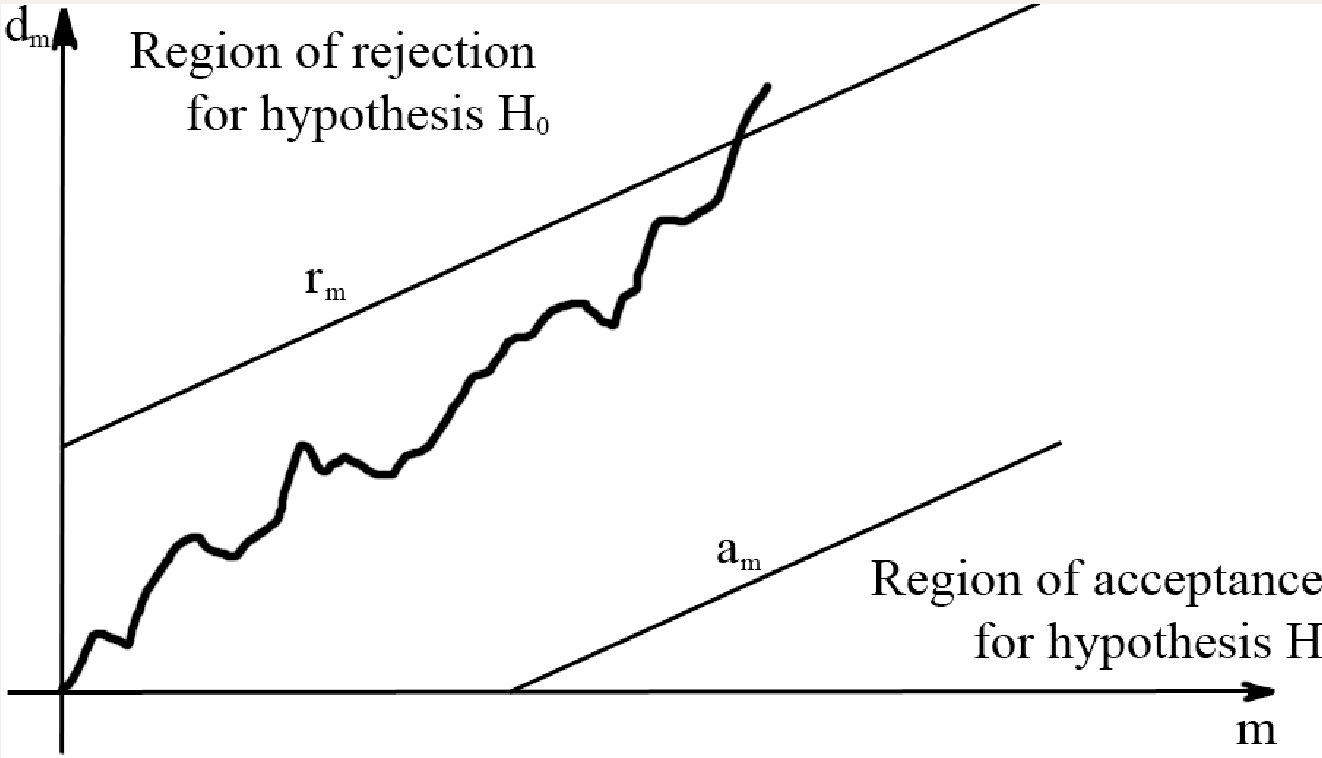
\includegraphics[width=0.6\textwidth]{wald1.png}
    \end{center}
    }
\end{frame}

\begin{frame}{Момент остановки}
    На каком элементы выборки $n$ произойдёт остановка процедуры?

    \bigskip

    $n$~--- случайная величина, можно говорить о её матожидании:
    $$\mathbb{E}_p\left(n\right) = \frac{L\left(p\right)\ln B + \left(1-L\left(p\right)\right)\ln A}{p \ln \frac{p_U}{p_L} + \left(1-p\right)\ln\frac{1-p_U}{1-p_L}},$$
    $L\left(p\right) = \frac{A^h-1}{A^h-B^h}$ --- оперативная характеристика --- вероятность принять нулевую гипотезу при~условии, что $p$~--- иcтинное значение параметра; 
    
    $h$ определяется как решение уравнения:
    $$p=\frac{1-\left(\frac{1-p_U}{1-p_L}\right)^h}{\left(\frac{p_U}{p_L}\right)^h-\left(\frac{1-p_U}{1-p_L}\right)^h}.$$
    \begin{center}
    \includegraphics[width=0.15\textwidth]{wald3.eps}
    \end{center}
\end{frame}

\begin{frame}{Усечение}
    Если при $m = n_0$ решение ещё не принято, но возможности добавлять элементы выборки больше нет, используем следующий критерий:
    \begin{itemize}
    \item $d_m\geq \frac{a_{n_0} + r_{n_0}}{2} \Rightarrow$ отвергаем $H_0,\;\; p\geq p_U;$
    \item $d_m\leq \frac{a_{n_0} + r_{n_0}}{2} \Rightarrow$ принимаем $H_0,\;\; p\leq p_L$.
    \end{itemize}

    \bigskip

    \begin{center}
    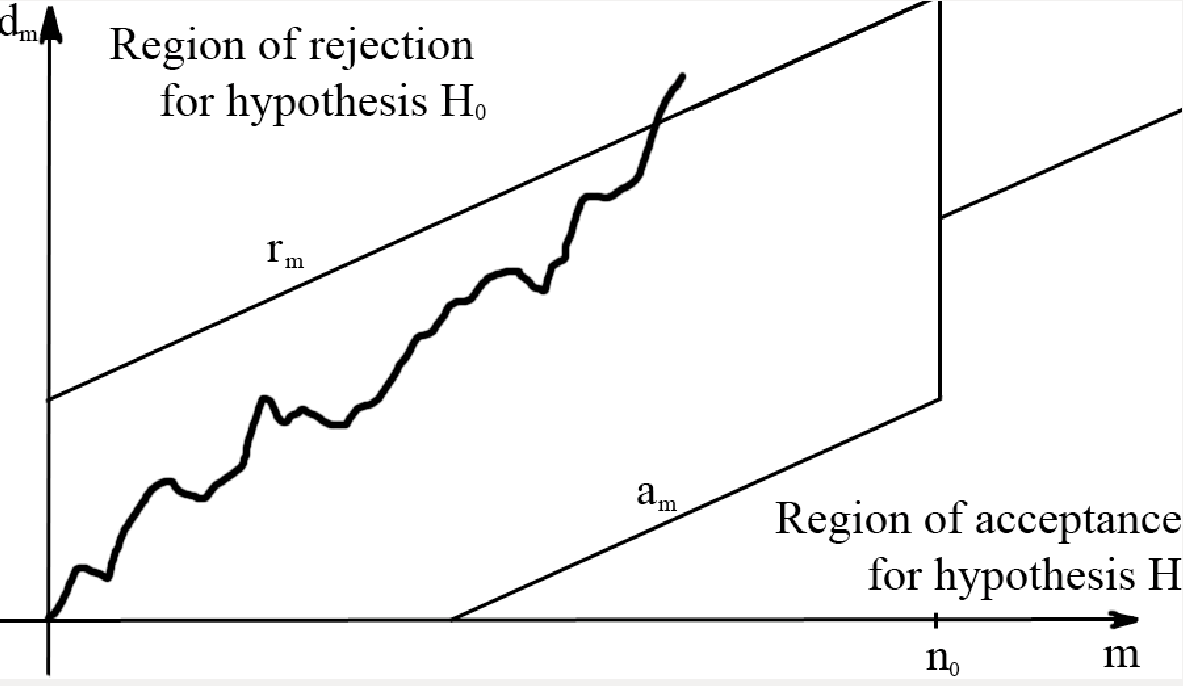
\includegraphics[width=0.6\textwidth]{wald2.png}
    \end{center}
\end{frame}

\begin{frame}{Группировка наблюдений}
    Наблюдения могут поступать группами $g_1, g_2, \dots$ по $v$ элементов.
    Тогда значения статистики $d_m$ сравниваются с $a_m, r_m$ только при $m = v, 2v, \dots$.

    \bigskip

    Последствия:
    \begin{itemize}
    \item увеличивается размер выборки, при котором происходит остановка;
    \item истинные вероятности ошибок могут оказаться больше номинальных, но при этом
        $$\alpha'\leq\frac{\alpha}{1-\beta}, \;\; \beta'\leq\frac{\beta}{1-\alpha}.$$
        Так как величины $\alpha$ и $\beta$ обычно малы, отклонением можно пренебречь.
    \end{itemize}
\end{frame}

\begin{frame}{Z-критерий для разности двух долей, связанные выборки}
     \only<1>{
%		\vspace{-12pt}
%		\small
		\begin{center}
			\begin{tabular}{rl}
            выборки:                        & $X_1^n=\left(X_{11},\ldots,X_{1n}\right), X_{1} \sim Ber\left(p_1\right)$ \\
                                            & $X_2^n=\left(X_{21},\ldots,X_{2n}\right), X_{2} \sim Ber\left(p_2\right)$ \\
                                            & выборки связанные
				
				\vspace{5pt}
				
				\\
				\multicolumn{2}{c}{     \begin{tabular}{|c|c|c|}
						\hline
						{$X_1^n$}{$X_2^n$}& 1     & 0   \\\hline
						1                              & $e$   & $f$  \\\hline
						0                              & $g$   & $h$  \\\hline
					\end{tabular}
					
					\vspace{5pt}
					
				} \\
				нулевая гипотеза:               & $H_0\colon p_1\geq p_2$ \\
				альтернатива:                   & $H_1\colon p_1<p_2$ \\
				статистика:                     & $Z\left(X_1^n, X_2^n\right) = \frac{f-g}{\sqrt{f+g-\frac{\left(f-g\right)^2}{n}}}$ \\
				нулевое распределение:          & $N(0,1)$ при $p_1=p_2$
			\end{tabular}
			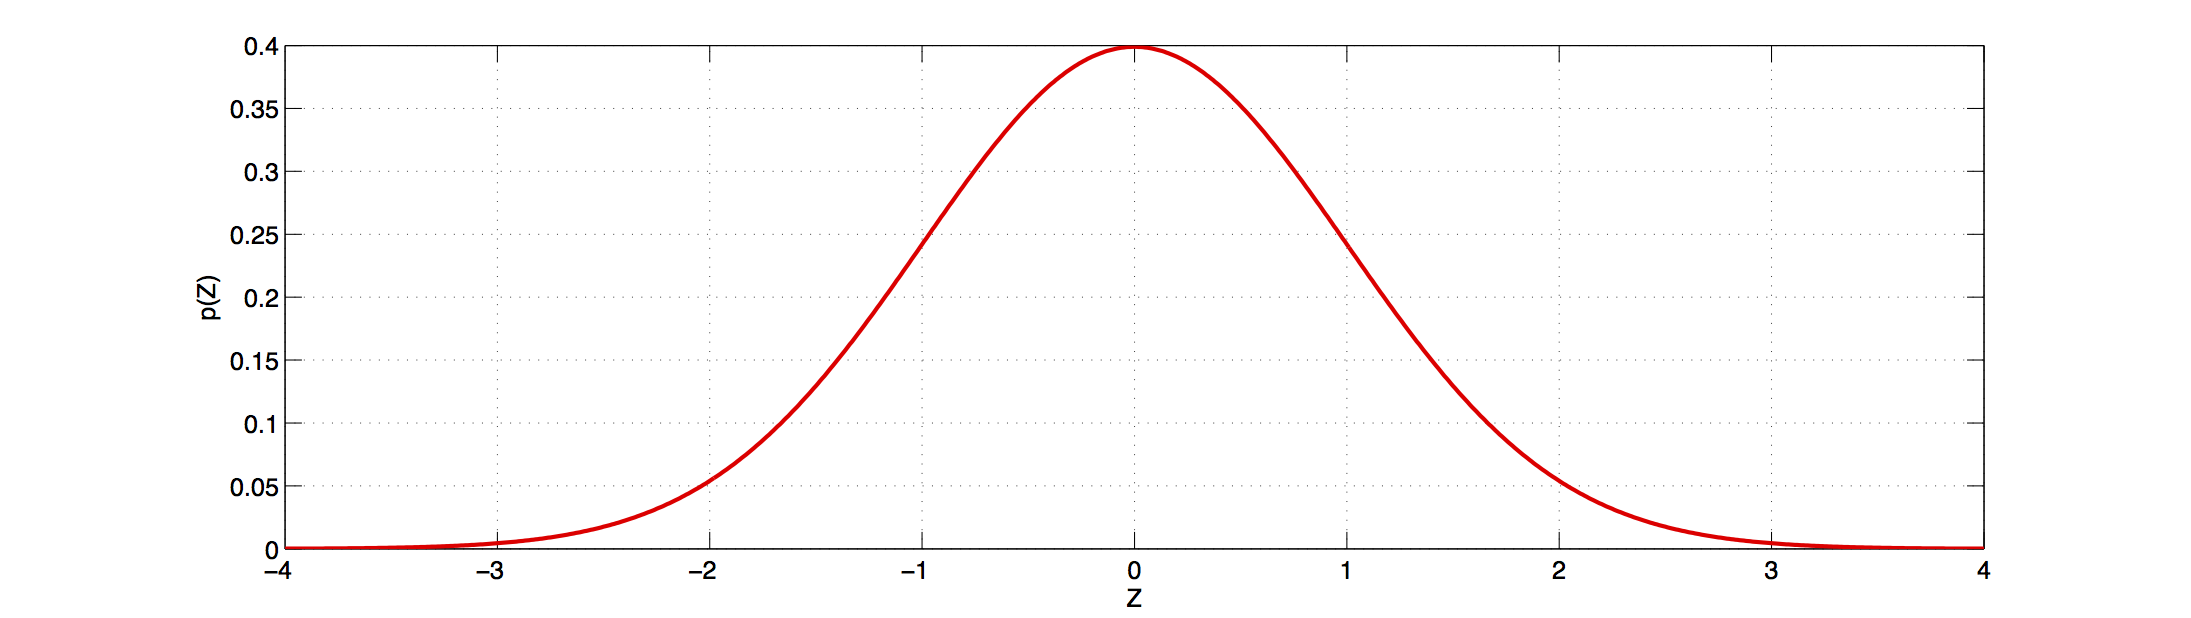
\includegraphics[width=0.8\textwidth]{norm.png}
		\end{center}
     }

     \only<2>{
     \textbf{Пример:} имеются два технологических процесса, классический и~модернизированный, $p_1, p_2$~--- доли брака в них.

     \bigskip

    $H_0\colon$ доля брака в классическом процессе не меньше доли брака в~модернизированном.

    $H_1\colon$ доля брака в классическом процессе меньше доли брака в~модернизированном.
     }
\end{frame}

\begin{frame}{Аналог в последовательном анализе}
    \only<1>{
    Пусть значения $x_{1i},x_{2i}$ поступают парами.

    Будем рассматривать только различающиеся пары~--- $(0,1)$ и $(1,0)$, а~остальные будем отбрасывать.

    \bigskip

    $k_1 = \frac{p_1}{1-p_1}, \; k_2 = \frac{p_2}{1-p_2}$~--- риски,

    $u=\frac{k_1}{k_2} = \frac{p_1\left(1-p_2\right)}{p_2\left(1-p_1\right)}$~--- относительный риск:
    \begin{itemize}
    \item $u=1 \; \Leftrightarrow \; p_1=p_2$,
    \item $u>1 \; \Leftrightarrow \; p_1>p_2$,
    \item $u<1 \; \Leftrightarrow \; p_1<p_2$.
    \end{itemize}
    Фиксируем <<коридор>> отклонений $u$ от 1, которые можно считать незначимыми:
    $$u_L\leq1\leq u_U$$
    (хотя бы одно из неравенств~--- строгое).

    \bigskip

       \begin{center}
        \begin{tabular}{rl}
            нулевая гипотеза:               & $H_0\colon u\geq u_U$ \\
            альтернатива:                   & $H_1\colon u\leq u_L$ \\
            статистика:                     & $d_m\left(X_1^{m},X_2^{m}\right) = \sum\limits_{i=1}^m \left(1-X_{1i}\right)X_{2i}$ \\
        \end{tabular}
   \end{center}
    }

    \only<2>{
    Константы последовательного анализа:
    $$a_m = \frac{\ln B + m \ln\frac{1+u_U}{1+u_L} }{ \ln u_U - \ln u_L},$$
    $$r_m = \frac{\ln A + m \ln\frac{1+u_U}{1+u_L} }{ \ln u_U - \ln u_L}.$$

    \bigskip

    Момент остановки:
    $$\mathbb{E}_u\left(n\right) = \frac{L\left(u\right) \ln B + \left(1-L\left(u\right)\right) \ln A}{\frac{u}{u+1} \ln \frac{u_U\left(1+u_L\right)}{u_L\left(1+u_U\right)} + \frac1{u+1} \ln \frac{1+u_L}{1+u_U}} \Bigg/ \left(p_1\left(1-p_2\right)+p_2\left(1-p_1\right)\right),$$
    $$L\left(u\right) = \frac{A^h-1}{A^h-B^h},$$
    $h$ определяется как решение уравнения
    $$\frac{u}{u+1} = \frac{1 - \left(\frac{1+u_L}{1+u_U}\right)^h}{\left(\frac{u_U\left(1+u_L\right)}{u_l\left(1+u_U\right)}\right)^h-\left(\frac{1+u_L}{1+u_U}\right)^h}.$$
    }
\end{frame}

\begin{frame}{Группировка наблюдений}
    Наблюдения могут поступать группами $g_1, g_2, \dots$ пар выборок по $v$~элементов.
    Если при этом внутри пар выборок не указаны соответствия элементов $(x_{1i}, x_{2i})$, статистику $d_m$ вычислить невозможно.

    \bigskip

    Пусть $v_1\left(g_i\right)$~--- число успехов в выборке из $v$ наблюдений над первой биномиальной совокупностью в группе $g_i$, $v_2(g_i)$~--- над второй.
    Тогда для этой пары групп в качестве оценки числа пар $(0,1)$ примем величину $v_2(g_i)-\frac{v_1\left(g_i\right)v_2\left(g_i\right)}{v}.$
    $$d_{g_m} = \sum_{i=1}^{g_m} \left(v_2(g_i)-\frac{v_1\left(g_i\right)v_2\left(g_i\right)}{v}\right).$$

    \bigskip

    Последствия: аналогичные.
\end{frame}

\section{Нормальное распределение}
\subsection{Среднее, односторонняя альтернатива}
\begin{frame}{Z-критерий для среднего нормального распределения, односторонняя альтернатива}
    \only<1>{
    \begin{center}
        \begin{tabular}{rl}
            выборка:                        & $X^n=\left(X_1,\ldots,X_n\right), X \sim N\left(\mu, \sigma^2\right), \sigma$ известна\\
            нулевая гипотеза:               & $H_0\colon \mu\leq\mu_0$ \\
            альтернатива:                   & $H_1\colon \mu>\mu_0$ \\
            статистика:                     & $Z\left(X^n\right) = \frac{\bar{X}-\mu_0}{\sigma / \sqrt{n}}$ \\
            нулевое распределение:          & $N(0,1)$ при $\mu=\mu_0$
        \end{tabular}
        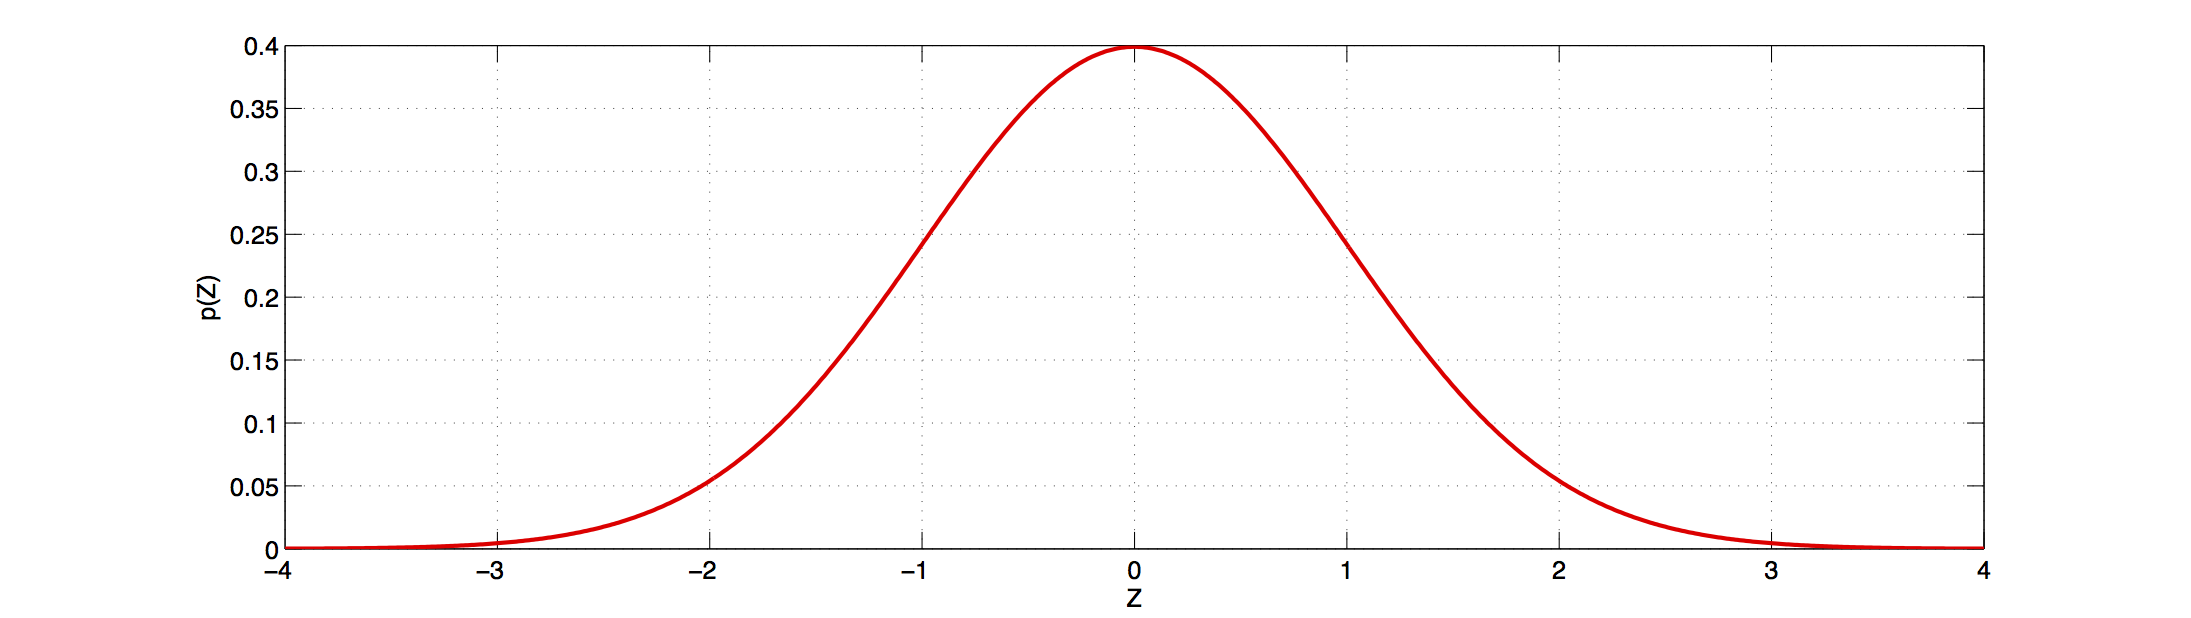
\includegraphics[width=0.8\textwidth]{norm.png}
    \end{center}
     }

     \only<2>{
     \textbf{Пример:} при помощи прибора с известной погрешностью $\sigma$ измеряется концентрация вредного вещества в образце. Необходимо проверить, что она не превышает предельно допустимой.
     }
\end{frame}

\begin{frame}{Аналог в последовательном анализе}
    \only<1>{
    Фиксируем <<коридор>> отклонений $\mu$ от $\mu_0$, которые можно считать незначимыми:
    $$\mu_L\leq\mu_0\leq \mu_U$$
    (хотя бы одно из неравенств~--- строгое).

    \bigskip

    \begin{center}
        \begin{tabular}{rl}
            нулевая гипотеза:               & $H_0\colon \mu\leq \mu_L$ \\
            альтернатива:                   & $H_1\colon \mu\geq \mu_U$ \\
            статистика:                     & $d_m\left(X^{m}\right) = \sum\limits_{i=1}^m X_{i}$ \\
        \end{tabular}
    \end{center}
    }

    \only<2>{
    Константы последовательного анализа:
    $$a_m = \frac{\sigma^2}{\mu_U-\mu_L}\ln B + m \frac{\mu_U+\mu_L}{2},$$
    $$r_m = \frac{\sigma^2}{\mu_U-\mu_L}\ln A + m \frac{\mu_U+\mu_L}{2},$$

    \bigskip

    Момент остановки:
    $$\mathbb{E}_{\mu}\left(n\right) = \frac{L(\mu)\ln B \left(1-L(\mu)\right)\ln A}{\mu_L^2-\mu_U^2 + 2\left(\mu_U-\mu_L\right)\mu},$$
    $$L\left(\mu\right) = \frac{A^h-1}{A^h-B^h},$$
    $$h=\frac{\mu_U+\mu_L-2\mu}{\mu_U-\mu_L}.$$
    }
\end{frame}

\subsection{Среднее, двусторонняя альтернатива}
\begin{frame}{Z-критерий для среднего нормального распределения, двусторонняя альтернатива}
    \only<1>{
    \begin{center}
        \begin{tabular}{rl}
            выборка:                        & $X^n=\left(X_1,\ldots,X_n\right), X \sim N\left(\mu, \sigma^2\right), \sigma$ известна\\
            нулевая гипотеза:               & $H_0\colon \mu=\mu_0$ \\
            альтернатива:                   & $H_1\colon \mu\neq\mu_0$ \\
            статистика:                     & $Z\left(X^n\right) = \frac{\bar{X}-\mu_0}{\sigma / \sqrt{n}}$ \\
            нулевое распределение:          & $N(0,1)$\\
        \end{tabular}
        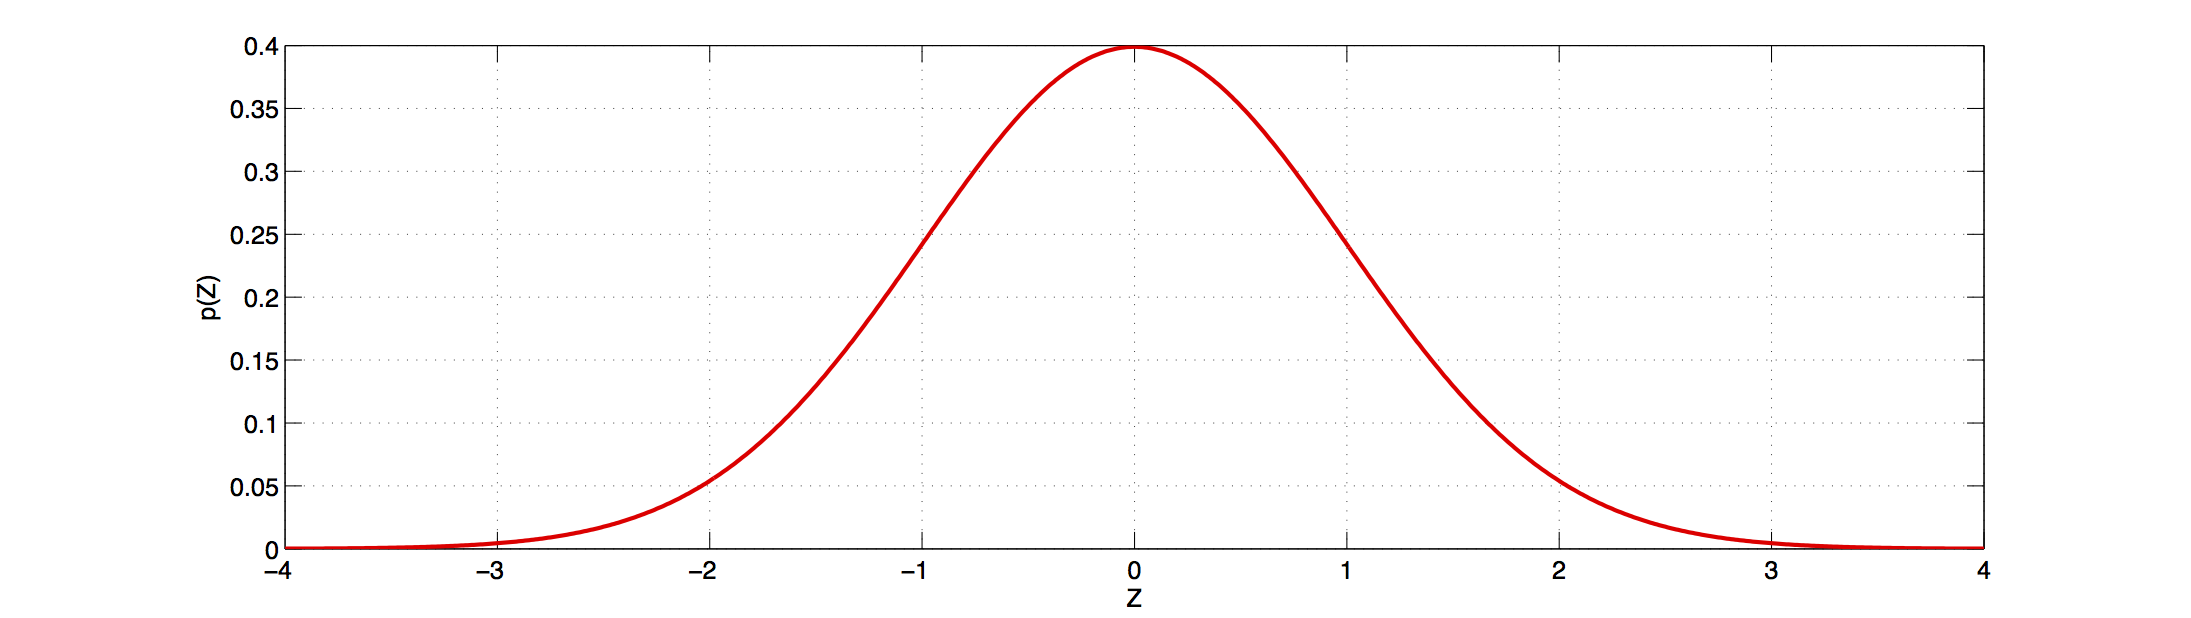
\includegraphics[width=0.8\textwidth]{norm.png}
    \end{center}
     }

     \only<2>{
     \textbf{Пример:} многократные измерения прибором с известной погрешностью для проверки наличия у прибора смещения.
     }
\end{frame}

\begin{frame}{Аналог в последовательном анализе}
    Фиксируем симметричный <<коридор>> отклонений $\mu$ от $\mu_0$, которые можно считать незначимыми:
    $$\left|\frac{\mu-\mu_0}{\sigma}\right|\leq\delta.$$

    \bigskip

    \begin{center}
        \begin{tabular}{rl}
            нулевая гипотеза:               & $H_0\colon \left|\frac{\mu-\mu_0}{\sigma}\right|\leq\delta$ \\
            альтернатива:                   & $H_1\colon \left|\frac{\mu-\mu_0}{\sigma}\right|>\delta$ \\
            статистика:                     & $d_m\left(X^{m}\right) = \ln \ch \left(\frac{\delta}{\sigma}\sum\limits_{i=1}^m \left(X_{i}-\mu_0\right)\right)$ \\
        \end{tabular}
    \end{center}

    \bigskip

    Константы последовательного анализа:
    $$a_m = \ln B +m\frac{\delta^2}{2},$$
    $$r_m = \ln A +m\frac{\delta^2}{2}.$$
\end{frame}

\subsection{Дисперсия}
\begin{frame}{Критерий хи-квадрат}
    \only<1>{
    \begin{center}
        \begin{tabular}{rl}
            выборка:                        & $X^n=\left(X_1,\ldots,X_n\right), X\sim N\left(\mu, \sigma^2\right), \mu$ известно\\
            нулевая гипотеза:               & $H_0\colon \sigma\leq\sigma_0$ \\
            альтернатива:                   & $H_1\colon \sigma>\sigma_0$ \\
            статистика:                     & $\chi^2\left(X^n\right) = \frac{\sum_{i=1}^n \left(X_i-\mu\right)}{\sigma_0^2}$ \\
            нулевое распределение:          & $\chi^2_n$ при $\sigma=\sigma_0$
        \end{tabular}
        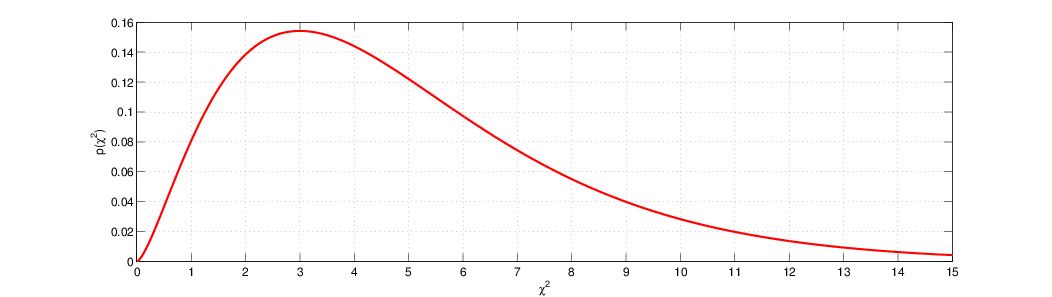
\includegraphics[width=0.8\textwidth]{chi2.png}
    \end{center}
     }

     \only<2>{
     \textbf{Пример:} не превышает ли погрешность прибора заявленного уровня?
     }
\end{frame}

\begin{frame}{Аналог в последовательном анализе}
    Фиксируем <<коридор>> отклонений $\sigma$ от $\sigma_0$, которые можно считать незначимыми:
    $$\sigma_L\leq\sigma_0\leq \sigma_U$$
    (хотя бы одно из неравенств~--- строгое).

    \bigskip

    \begin{center}
        \begin{tabular}{rl}
            нулевая гипотеза:               & $H_0\colon \sigma\leq \sigma_L$ \\
            альтернатива:                   & $H_1\colon \sigma\geq \sigma_U$ \\
            статистика:                     & $d_m\left(X^{m}\right) = \sum\limits_{i=1}^m \left(X_{i}-\mu\right)^2$ \\
        \end{tabular}
    \end{center}

    \bigskip

    Константы последовательного анализа:
    $$a_m = \frac{2\ln B + m \ln \frac{\sigma^2_U}{\sigma^2_L}}{\frac1{\sigma^2_L} - \frac1{\sigma^2_U}},$$
    $$r_m = \frac{2\ln A + m \ln \frac{\sigma^2_U}{\sigma^2_L}}{\frac1{\sigma^2_L} - \frac1{\sigma^2_U}}.$$
\end{frame}

\begin{frame}{Случай неизвестного среднего}
    Если среднее неизвестно, предлагается использовать его выборочную оценку:
    \begin{center}
        \begin{tabular}{rl}
            статистика:                     & $d_m\left(X^{m}\right) = \sum\limits_{i=1}^m \left(X_{i}-\bar{X}\right)^2$ \\
        \end{tabular}
    \end{center}

    При этом в последовательном анализе на $m$-м шаге вместо констант $a_m, r_m$ необходимо использовать $a_{m-1}, r_{m-1}$.
\end{frame}


\subsection{Последовательные доверительные интервалы}
\begin{frame}{Доверительный интервал для среднего}
    Дано: $X_1,\dots,X_n, \;\; X\sim N\left(\mu, \sigma^2\right),$ \; $\mu, \sigma$ неизвестны.
    
    \bigskip
    
    Требуется: построить доверительный интервал $J$ для среднего $\mu$ фиксированной длины $2d$: $$P\left(\mu\in J\right)\geq 1-\alpha \;\; \forall \mu, \sigma.$$    
    
    \bigskip
    
    При фиксированном $n$ и неизвестном $\sigma$ решения не существует (Данциг, 1940).
\end{frame}

\begin{frame}{Последовательные доверительные интервалы для среднего}
    \only<1>{
    При известном $\sigma$:
    $$J_n = \left[\bar{X}_n - d, \bar{X}_n + d\right], $$
    $$P\left(\mu \in J_n\right) = P\left(\left|\bar{X}_n-\mu\right|\leq d\right) = P\left(\frac{\sqrt{n}\left|\bar{X}_n-\mu\right|}{\sigma} \leq \frac{\sqrt{n}d}{\sigma}\right) = 2\Phi\left(\sqrt{n}d/\sigma\right)-1;$$       
    $$2\Phi\left(\sqrt{n}d/\sigma\right)-1 \geq 1-\alpha = 2\Phi\left(z_{1-\alpha/2}\right)-1;$$
    так как $\Phi$ монотонна, 
    $$\frac{\sqrt{n}d}{\sigma} \geq z_{1-\alpha/2} \Rightarrow n \geq \frac{z_{1-\alpha/2}^2 \sigma^2}{d^2} \equiv C.$$
    $C$~--- минимальный размер выборки, при котором $J_n$ имеет уровень доверия $1-\alpha$.
    }
    
    \only<2>{
    \textbf{Двухэтапная процедура Стейна}.
    \begin{enumerate}
    \item $X_1,\dots,X_m$~--- пилотная выборка, $m\geq 2,$ \; $S_m^2$~--- её выборочная дисперсия.
    \item Определим, сколько нужно добавить наблюдений:
    	  \begin{align*}
    	  \hat{C} &= \frac{t^2_{1-\alpha/2, m-1}S_m^2}{d^2}, \\
    	  N       &= \max \left(\left[\hat{C}\right]+1, m\right),
    	  \end{align*}
    	  $J_N =\left[\bar{X}_N - d, \bar{X}_N + d\right]$~--- искомый $100(1-\alpha)$\% доверительный интервал для $\mu$. 
    \end{enumerate}
    
    \bigskip
    
    $$\frac{t^2_{1-\alpha/2, m-1}}{z_{1-\alpha/2}^2} C \leq \mathbb{E}_{\mu,\sigma}\left(N\right) \leq \frac{t^2_{1-\alpha/2, m-1}}{z_{1-\alpha/2}^2} C + m.$$
    }
    
    \only<3>{
    Двухэтапная процедура состоятельна:
    $$P_{\mu,\sigma} \left(\mu \in J_N\right)\geq 1-\alpha,$$
    
    и асимптотически состоятельна:
    $$\lim\limits_{d\rightarrow 0 } P_{\mu,\sigma} \left(\mu \in J_N\right) = 1-\alpha,$$
    
    но асимптотически неэффективна:
    $$\lim\limits_{d\rightarrow 0 } \mathbb{E}_{\mu,\sigma} \left(\frac{N}{C}\right)= \frac{ t^2_{1-\alpha/2, m-1}}{z^2_{1-\alpha/2}}>1.$$
    }
    
    \only<4>{
    \textbf{Полностью последовательная процедура}.
    \begin{itemize}
    \item $X_1,\dots,X_m$~--- пилотная выборка, $m\geq 2.$
    \item Для каждого $n=m,m+1,\dots$  вычисляем $$\hat{C}_n = \frac{z^2_{1-\alpha/2}S_n^2}{d^2}.$$
    \item Продолжаем набирать выборку, если $n < \hat{C}_n$.
    \end{itemize}
        
    \bigskip
    
    $N$~--- наименьшее целое $n\geq \hat{C}_n$.
    $$\mathbb{E}_{\mu,\sigma}\left(N\right) \leq C+m.$$
    }
    
    \only<5>{
    Полностью последовательная процедура только асимптотически состоятельна:
    $$\lim\limits_{d\rightarrow 0 } P_{\mu,\sigma} \left(\mu \in J_N\right) = 1-\alpha,$$
    
    но зато асимптотически эффективна:
    $$\lim\limits_{d\rightarrow 0 } \mathbb{E}_{\mu,\sigma} \left(\frac{N}{C}\right)= 1.$$
    }    
\end{frame}

\begin{frame}{Доверительный интервал для разности двух средних}
    Дано: $X_{i1},\dots,X_{in_i}, \;\; X_i \sim N\left(\mu_i, \sigma_i^2\right),$ \; $i=1,2.$ 
    
    \bigskip
    
    Требуется: построить доверительный интервал $J$ для разности средних $\mu_1-\mu_2$ фиксированной длины $2d$:
     $$P\left(\mu_1-\mu_2\in J\right)\geq 1-\alpha \;\; \forall \mu_1,\mu_2, \sigma_1,\sigma_2.$$
     
     \bigskip
     
     Введём следующие обозначения:
     \begin{align*}
     n     &= \left(n_1,n_2\right), \\
     T_n   &= \bar{X}_{1n_1} -  \bar{X}_{2n_2}, \\
     U_n^2 &= \frac{\left(n_1-1\right)S_{1n_1}^2 + \left(n_2-1\right)S_{2n_2}^2}{n_1+n_2-2}.
     \end{align*}
     
     \bigskip
     
     Будем рассматривать доверительные интервалы $J_n = \left[T_n-d, T_n+d\right]$.
\end{frame}

\begin{frame}{Случай $\sigma_1=\sigma_2=\sigma$}
    \only<1>{
    Поскольку дисперсии равны, будем брать выборки одинакового размера:
    \begin{align*}
    n_1&=n_2=n, \\
    U_n^2 &= \frac{S_{1n}^2 + S_{2n}^2}{2}.
    \end{align*}
    
    \bigskip
    
    \textbf{Двухэтапная процедура}.
    \begin{enumerate}
    \item $X_{i1},\dots,X_{im}$~--- пилотные выборки, $m\geq 2,$ \; $U_m^2$~--- оценка дисперсии по ним.
    \item Определим, сколько нужно добавить пар наблюдений:
		    \begin{align*}
				\hat{C} &= \frac{2 t^2_{1-\alpha/2, 2m-2}U_m^2}{d^2}, \\
				N       &= \max \left(\left[\hat{C}\right]+1, m\right), 
		    \end{align*}
    	  $J_N =\left[\bar{T}_N - d, \bar{T}_N + d\right]$~--- искомый $100(1-\alpha)$\% доверительный интервал для $\mu_1-\mu_2$. 
    \end{enumerate}
    }
    
    \only<2>{
    $$\frac{t^2_{1-\alpha/2, 2m-2}}{z_{1-\alpha/2}^2} C \leq \mathbb{E}_{\mu_1, \mu_2,\sigma}\left(N\right) \leq \frac{t^2_{1-\alpha/2, 2m-2}}{z_{1-\alpha/2}^2} C + m.$$    
    
    \bigskip
    
    Двухэтапная процедура состоятельна и асимптотически состоятельна, но~асимптотически неэффективна (по сравнению с $C=\frac{2z_{1-\alpha/2}^2\sigma^2}{d^2}$).
    }
\end{frame}

\begin{frame}{Случай $\sigma_1\neq\sigma_2$}
    \only<1>{
    Пусть $W_1,W_2\sim St\left(m-1\right)$ независимы, $h_{m,1-\alpha/2}$~--- $(1-\alpha/2)$-квантиль распределения $W_1-W_2$:
    $$P\left(W_1-W_2\leq h_{m,1-\alpha/2}\right) = 1 - \frac{\alpha}{2}.$$
    $h_{m,1-\alpha/2} \approx \sqrt{2} z_{1-\alpha/2}.$
    \bigskip
    
    \textbf{Двухэтапная процедура}.
	\begin{enumerate}
    \item $X_{i1},\dots,X_{im}$~--- пилотные выборки, $m\geq 2,$ \; $S_{1m}^2, S_{2m}^2$~--- оценки дисперсий по ним;
    \item Определим, сколько нужно добавить наблюдений в каждую выборку:
    	  \begin{align*}
    	  \hat{C}_1 = \frac{h_{m,1-\alpha/2} S_{1m}^2}{d^2}, \;\;&\;\; \hat{C}_2 = \frac{h_{m,1-\alpha/2} S_{2m}^2}{d^2}, \\
    	  N_1 = \max \left(\left[\hat{C}_1\right]+1, m\right),\;\; &\;\; N_2 = \max \left(\left[\hat{C}_2\right]+1, m\right),
    	  \end{align*}
    	  $J_N =\left[\bar{T}_N - d, \bar{T}_N + d\right],$ \; $N=\left(N_1,N_2\right)$~--- искомый $100(1-\alpha)$\% доверительный интервал для $\mu_1-\mu_2$. 
    \end{enumerate}
    }
    
    \only<2>{   
    $$\mathbb{E}N_i \approx \frac{h^2_{m, 1-\alpha/2} \sigma_i^2}{d^2}, \; i=1,2.$$
    
    \bigskip
    
    Двухэтапная процедура состоятельна.
    
    \bigskip
    
    В рамках последовательного анализа удалось найти точное решение проблемы Беренца-Фишера!    
    }
    \iffalse
    \only<3>{
    \textbf{Полностью последовательная процедура}.
    \begin{itemize}
    \item $X_{i1},\dots,X_{im}$~--- пилотные выборки, $m\geq 2.$
    \item Продолжаем набирать первую выборку, если $\frac{n_1}{n_2} \leq \frac{S_{1n_1}}{S_{2n_2}}$, и вторую, если $\frac{n_1}{n_2} > \frac{S_{1n_1}}{S_{2n_2}}$.
    \item Останавливаемся по одному из трёх правил:
    \begin{align}
    & n_1+n_2 \geq \frac{z^2_{1-\alpha/2}}{d^2}\left(S_{1n_1} + S_{2n_2}\right)^2, \\
    & \frac{S^2_{1n_1}}{n_1} + \frac{S^2_{2n_2}}{n_2} \leq \frac{d^2}{z^2_{1-\alpha/2}}, \\
    & \left\{ \begin{aligned}
    	n_1&\geq \frac{z^2_{1-\alpha/2}}{d^2}S_{1n_1}\left(S_{1n_1} + S_{2n_2}\right), \\
    	n_2&\geq \frac{z^2_{1-\alpha/2}}{d^2}S_{2n_2}\left(S_{1n_1} + S_{2n_2}\right).
      \end{aligned} \right.
    \end{align}
    \end{itemize}
    }
    
    \only<4>{
    Пусть $N_1,N_2$~--- объёмы выборок, при которых произошла остановка, $N=N_1+N_2$.
    
    $$\mathbb{E}_{\mu_1,\mu_2,\sigma_1, \sigma_2}\left(N\right) \leq C + m + 2.$$
    
    \bigskip
    
    Для $N^{(1)}, N^{(2)}, N^{(3)}$~--- суммарных объёмов выборок, при которых произошла остановка с использованием правил (1), (2) и (3)~--- справедливо $$N^{(1)}\leq N^{(2)}\leq N^{(3)}.$$
    
    \bigskip    
    
     Полностью последовательная процедура асимптотически состоятельна и~асимптотически эффективна (относительно $C=\frac{z^2_{1-\alpha/2}}{d^2}\left(\sigma_1+\sigma_2\right)^2.$).       
    }
    \fi
\end{frame}

\section{Непараметрическое оценивание}
\subsection{Непараметрическое оценивание матожидания}
\begin{frame}{Доверительный интервал для матожидания}
    Дано: $X_1,X_2,\dots, \;\; X\sim F\left(x\right),$ \; $\mathbb{E}X,$\;$\mathbb{D}X$ конечны.
    
    \bigskip
    
    Требуется: построить доверительный интервал $J$ для среднего $\mathbb{E}X$ фиксированной длины $2d$: 
    $$P\left(\mathbb{E}X \in J\right)\geq 1-\alpha \;\; \forall F\left(x\right).$$    
    
    \bigskip
    
    Если известно $\mathbb{D}X$, по центральной предельной теореме приближённым решением является интервал $J_n=\left[\bar{X}_n-d,\bar{X}_n+d\right],$ где $n$~--- наименьшее целое, удовлетворяющее условию $$n \geq \frac{z_{1-\alpha/2} \left(\mathbb{D}X\right)^2}{d^2} \equiv C.$$
\end{frame}

\begin{frame}{Последовательные доверительные интервалы для матожидания}
	\textbf{Полностью последовательная процедура}.
    \begin{itemize}
    \item $X_{1},\dots,X_{m}$~--- пилотная выборка, $m\geq 2,$ \; $S_m^2$~--- оценка дисперсии по ней.
    \item Для каждого $n=m,m+1,\dots$ вычисляем $$\hat{C}_n = \frac{z^2_{1-\alpha/2}\left(S_n^2+\frac1{n}\right)}{d^2}.$$
    \item Продолжаем набирать выборку, если $n < \hat{C}_n$.
    \end{itemize}
	$\frac1{n}$~--- поправка на случай, если распределение $F\left(x\right)$ дискретно.
	
	\bigskip
	
	$N$~--- наименьшее целое $n\geq \hat{C}_n$.
	$$\mathbb{E}_{F}\left(N\right) \leq C + m + 2.$$
	
	Процедура асимптотически состоятельна и~асимптотически эффективна.
\end{frame}

\subsection{Непараметрическое оценивание медианы}
\begin{frame}{Доверительный интервал для медианы}
    \only<1>{
    Дано: $X_1,X_2,\dots, \;\; X\sim F\left(x-\theta\right),$ \; $\theta=\med X,$
    \begin{itemize}
    \item $F\left(x\right)$ симметрична относительно нуля,
    \item $F\left(x\right)$ дважды дифференцируема в окрестности нуля $\mathcal{N}$;
    \item $F''\left(x\right)$ ограничена вне $\mathcal{N}$.
    \end{itemize}
    
    \bigskip
    
    Требуется: построить доверительный интервал $J$ для медианы $\theta$ фиксированной длины $2d$: 
    $$P\left(\theta \in J\right)\geq 1-\alpha \;\; \forall F\left(x\right).$$
    }
    \only<2>{
    При фиксированом $n$ асимптотический доверительный интервал задаётся порядковыми статистиками:
    \begin{align*}
    b(n) &= \max\left(1, \left[\frac1{2} \left(n-z_{1-\alpha/2} \sqrt{n} -1\right)\right]\right), \\
    a(n) &= n - b(n) + 1, \\
    J_n  &= \left[X_{n:b(n)}, X_{n:a(n)}\right], \\
    \lim_{n\rightarrow\infty}& P\left(\theta \in J_n\right) = 1-\alpha.
    \end{align*}
    
    \bigskip
    
    Чтобы построить доверительный интервал фиксированной длины $2d$ с~помощью полностью последовательной процедуры, нужно продолжать набирать выборку, пока $X_{n:a(n)} - X_{n:b(n)}>2d$.
%    
%    Такая процедура асимптотически состоятельна и~асимптотически эффективна (с $C=\frac{z_{1-\alpha/2}}{4d^2f^2(0)}$).
    }
\end{frame}

\begin{frame}{A/B тестирование}
\begin{block}{}
    Ваша компания производит газировку. Вы хотите предложить потребилтелям новый рецепт газировки, но не уверены, что он им понравится.    
\end{block}

\textbf{Решение:} A/B тест:
\begin{itemize}
    \item Половине потребителей дать газировку со старым рецептом, половине --- с новым.
    \item Проверить статистически, что люди активнее$^{*}$ выбирают новый рецепт.    
\end{itemize}
\end{frame}


\begin{frame}{A/B тестирование: общая схема}
\centering
%https://towardsdatascience.com/how-to-conduct-a-b-testing-3076074a8458
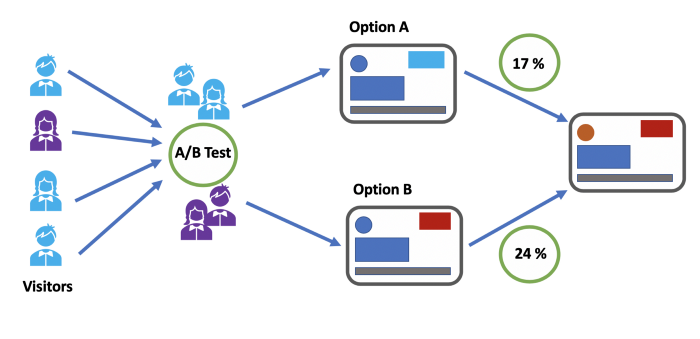
\includegraphics[width=0.75\textwidth]{ab.png}
(Kabir, 2020)
\end{frame}

\begin{frame}{A/B тестирование: особенности применения}
\begin{itemize}
\item Альтернатива фокус-группам, при правильной постановке задачи работает лучше (пример с газировкой)
\item Оффлайн-тестирование
\item Связность выборок: важен порядок!
\item Аналог плацебо: A/A тестирование
\item Для принятия решения используются ``метрики''
\end{itemize}
\end{frame}


\begin{frame}{A/B тестирование: ``метрики''}
\begin{itemize}
\item Выручка на пользователя (AVPRU): $t$-критерий;
\item Процент пользователей, кликнувших на ссылку (CTR): биномиальные критерии
\item Количество транзакций от пользователя
\item Количество покупок каждого продукта
\end{itemize}
\end{frame}

% https://blog.analytics-toolkit.com/2019/what-can-you-learn-from-running-an-a-b-test-for-2-years/
\begin{frame}{A/B тестирование и последовательный анализ}
\centering
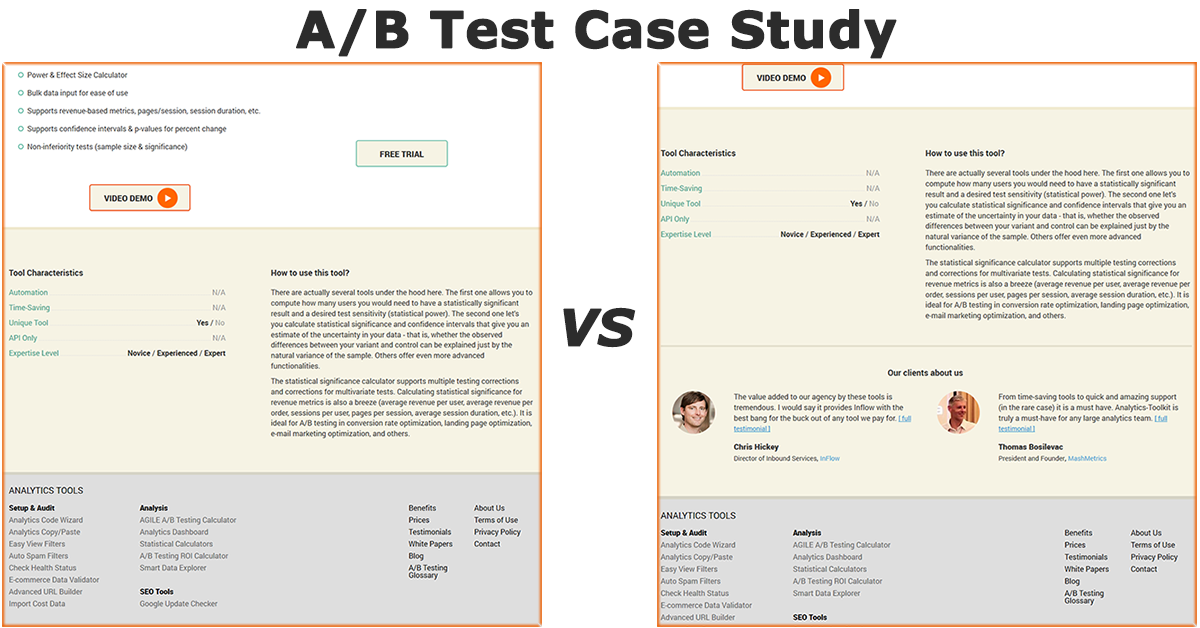
\includegraphics[width=0.75\textwidth]{ab2.png}
\end{frame}

\begin{frame}{A/B тестирование и последовательный анализ}
\centering
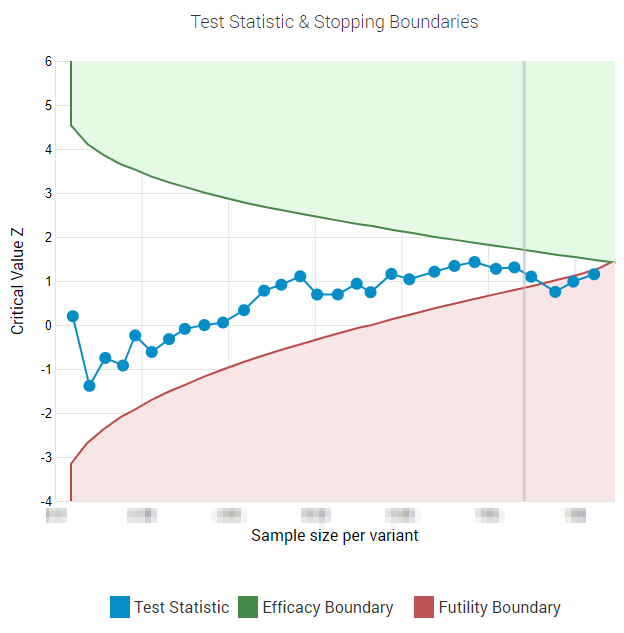
\includegraphics[width=0.5\textwidth]{ab3.png}
\end{frame}



\section{}
\begin{frame}{Литература}
    \begin{itemize}
    \item последовательная проверка гипотез --- Вальд;
    \item последовательные доверительные интервалы~--- Mukhopadhyay.
%    \item последовательный анализ для более сложных экспериментов~--- Rasch.
    \end{itemize}
	
	\bigskip
	
    {\small
    Вальд, А. {\em Последовательный анализ}, 1960.
	
	\bigskip
	
    Mukhopadhyay, N., de Silva, B. M. {\em Sequential methods and their applications}, 2009.
%    
%    Rasch D., Pilz J., Verdooren R., Gebhardt A. {\em Optimal Experimental Design with R}. --- Boca Raton: Chapman and Hall/CRC, 2011.
    }
\end{frame}

\begin{frame}{Литература}
    \begin{itemize}
    \item https://towardsdatascience.com/how-to-conduct-a-b-testing-3076074a8458
    \item https://blog.analytics-toolkit.com/2019/what-can-you-learn-from-running-an-a-b-test-for-2-years/

    \end{itemize}
\end{frame}



\end{document}
